\pdfoutput=1

\documentclass{article}
\usepackage{iclr2018}
\usepackage{times}
\usepackage{float}
\usepackage{hyperref}
\usepackage{url}
\usepackage{graphicx}
\usepackage{amsmath}
\usepackage{amsfonts}
\usepackage{subcaption}
\usepackage{listings}
\usepackage{lipsum}
\usepackage{microtype}
\usepackage{booktabs}
\usepackage{multirow}
\usepackage{siunitx}
\usepackage{hyphenat}

\usepackage{pifont}% http://ctan.org/pkg/pifont
\newcommand{\cmark}{\ding{51}}%
\newcommand{\xmark}{\ding{55}}%

\newcommand{\mixup}{\emph{mixup}}
\newcommand{\todo}[1]{{\color{red} TODO: {#1}}}
\DeclareMathOperator*{\E}{\mathbb{E}}
\newcommand*\samethanks[1][\value{footnote}]{\footnotemark[#1]}

\lstdefinestyle{mypython}{
  language=python,
  breaklines=true,
  basicstyle=\fontsize{8.5}{13}\selectfont\ttfamily,
  keywordstyle=\bfseries\color{green!40!black},
}

\iclrfinalcopy

\title{\mixup{}: Beyond Empirical Risk Minimization}

\author{%
Hongyi Zhang \\
MIT
\And
Moustapha Cisse, Yann N. Dauphin, David Lopez-Paz\thanks{Alphabetical order.} \\
FAIR
}

\begin{document}
    \maketitle
    \begin{abstract}
        Large deep neural networks are powerful, but exhibit undesirable
        behaviors such as memorization and sensitivity to adversarial examples.
        In this work, we propose \mixup{}, a simple learning principle to
        alleviate these issues. In essence, \mixup{} trains a neural network on
        convex combinations of pairs of examples and their labels.  By doing
        so, \mixup{} regularizes the neural network to favor simple linear
        behavior in-between training examples.  Our experiments on the
        ImageNet-2012, CIFAR-10, CIFAR-100, Google commands and UCI datasets
        show that \mixup{} improves the generalization of state-of-the-art
        neural network architectures.  We also find that \mixup{} reduces the
        memorization of corrupt labels, increases the robustness to adversarial
        examples, and stabilizes the training of generative adversarial
        networks.
    \end{abstract}
    %
\section{Introduction}
%
% Problem
Time series modeling is a well-established problem, with tasks such as forecasting and classification motivated by many domains such as healthcare, finance, and engineering~\citep{shumway2000time}. 
% Furthermore, time series data is diverse and readily available, presenting an exciting modality to learn from.
% Why interesting, important, and hard
However, effective time series modeling presents several challenges: 
% Methods often must be expressive, able to forecast arbitrary horizons, and efficient.
% itemsep=0.1pt,
\begin{itemize}[leftmargin=*]
% \begin{itemize}[itemsep=0.1pt, topsep=0pt,leftmargin=*]
\item First, 
% to effectively model time series data, 
methods should \textbf{expressively} capture complex, long-range, and \emph{autoregressive} dependencies. 
Time series data often reflects higher order dependencies, seasonality, and trends, governing how past samples determine future terms~\citep{chatfield2000time}. 
This motivates many classical approaches 
% and deep learning methods~\citep{zhou2022film, zhou2022fedformer, woo2022etsformer} 
that model these properties~\citep{box1970time, winters1960forecasting}, alongside expressive deep learning mechanisms such as attention~\citep{vaswani2017attention} and fully connected layers that model interactions between \emph{every} sample in an input sequence~\citep{zeng2022transformers}.
%
\item Second, 
% for forecasting, 
methods
% to tackle a wide range of time series data domains and tasks, 
% methods
should be able to forecast a wide range of \textbf{long horizons} over various data domains. 
% \eg{} to handle various forecasting horizons,
% and data domains,  
% methods should be (ii) \emph{broadly and easily applicable}, 
% without costly manual oversight or overly-specialized architectural changes. 
% without costly or overspecialized architectural changes. 
Reflecting real world demands, popular forecasting benchmarks evaluate methods on
% across 58 datasets with individual target horizons~\citep{godahewa2021monash} or 
\numberMonashTasks{} different tasks~\citep{godahewa2021monash} and 24$-$960 time-step horizons~\cite{zhou2021informer}. 
Furthermore, as testament to accurately learning time series processes, 
% as a test for learning time series,
forecasting methods should ideally
% should thus handle long horizons, and ideally 
% continuously 
also be able to predict future time-steps on horizons they were not explicitly trained on.
% ideally without the need for additional retraining and architectural adaptation. 
% with fixed input sequences. 
% Classification and forecasting methods should generalize to various datasets.
%
\item Finally, methods should be \textbf{efficient} with training and inference. Many time series applications require processing very long sequences, \eg{} classifying audio data with sampling rates up to $16{,}000$ Hz \citep{warden2018speech}. 
To handle such settings---where we still need large enough models that can expressively model this data---training and inference should ideally scale \emph{subquadratically} with sequence length and model size in time and space complexity.
% Efficient training over long sequences is a fundamental challenge for deep learning, where popular Transformers 
%To thus effectively learn from such time series on modern hardware, we require fast inference that fits memory constraints.
\end{itemize}

% Why prior stuff isn't sufficient
Unfortunately, existing time series methods struggle to achieve all three criteria.  
%
Classical methods (\cf{} ARIMA~\citep{box1970time}, exponential smoothing (ETS)~\citep{winters1960forecasting}) often require manual data preprocessing and model selection to identify expressive-enough models. 
%To effectively scale across all such evaluations, we ideally can avoid added complexities with a single simple architecture.
%
Deep learning methods commonly train to predict specific horizon lengths, \ie{} as \emph{direct multi-step forecasting}~\citep{https://doi.org/10.1111/j.1467-6419.2007.00518.x}, and we find this hurts their ability to forecast longer horizons (Sec. \ref{sec:empirical_horizons}).  
% On applicability, 
% state-of-the-art neural nets often introduce specialized architectures to handle specific data properties~\citep{liu2022pyraformer,zhou2022film}. 
%
They also face limitations achieving high expressivity \emph{and} efficiency. Fully connected networks (FCNs) such as NLinear \cite{zeng2022transformers} scale quadratically in $\mathcal{O}(\ell h)$ space complexity (with input length $\ell$ and forecast length $h$). 
%
Recent Transformer-based models reduce this complexity to $\mathcal{O}(\ell + h)$, but do not always outperform the aforementioned fully connected networks on forecasting benchmarks~\citep{liu2022pyraformer, zhou2021informer}. 
%

% , despite introducing various specific architectures to improve expressiveness or efficiency~\citep{ zhou2022film, zhou2022fedformer, woo2022etsformer}.
% However, they rarely obtain higher MSE over FCNs on benchmarks, and introduce various specific architectures and processing steps.


% Deep learning methods may be highly expressive but are either non-generic by adding specialized architectures to deal with different data properties (\eg{} trends, seasonality) and tasks (\eg{} classification, forecasting, forecasting with different horizons) or are not efficient at processing long sequences. For example, fully-connected networks in \cite{zeng2022transformers} are highly expressive and achieve state-of-the-art results on many forecasting benchmarks; however, their time and space complexity scales quadratically in input sequence length and forecast horizon length. Transformer variations bring down this complexity to near linear in compute and memory~\citep{liu2022pyraformer, zhou2021informer}; however, they rarely obtain higher MSE over FCNs on benchmarks, and introduce various specific architectures and processing steps~\citep{zhou2022film, zhou2022fedformer, woo2022etsformer}.

\begin{figure}[!t]
  \centering
%   \includegraphics[width=1\textwidth]{_ICLR2023_paper/figures/figure_pull_2layer_v1.2.pdf}
  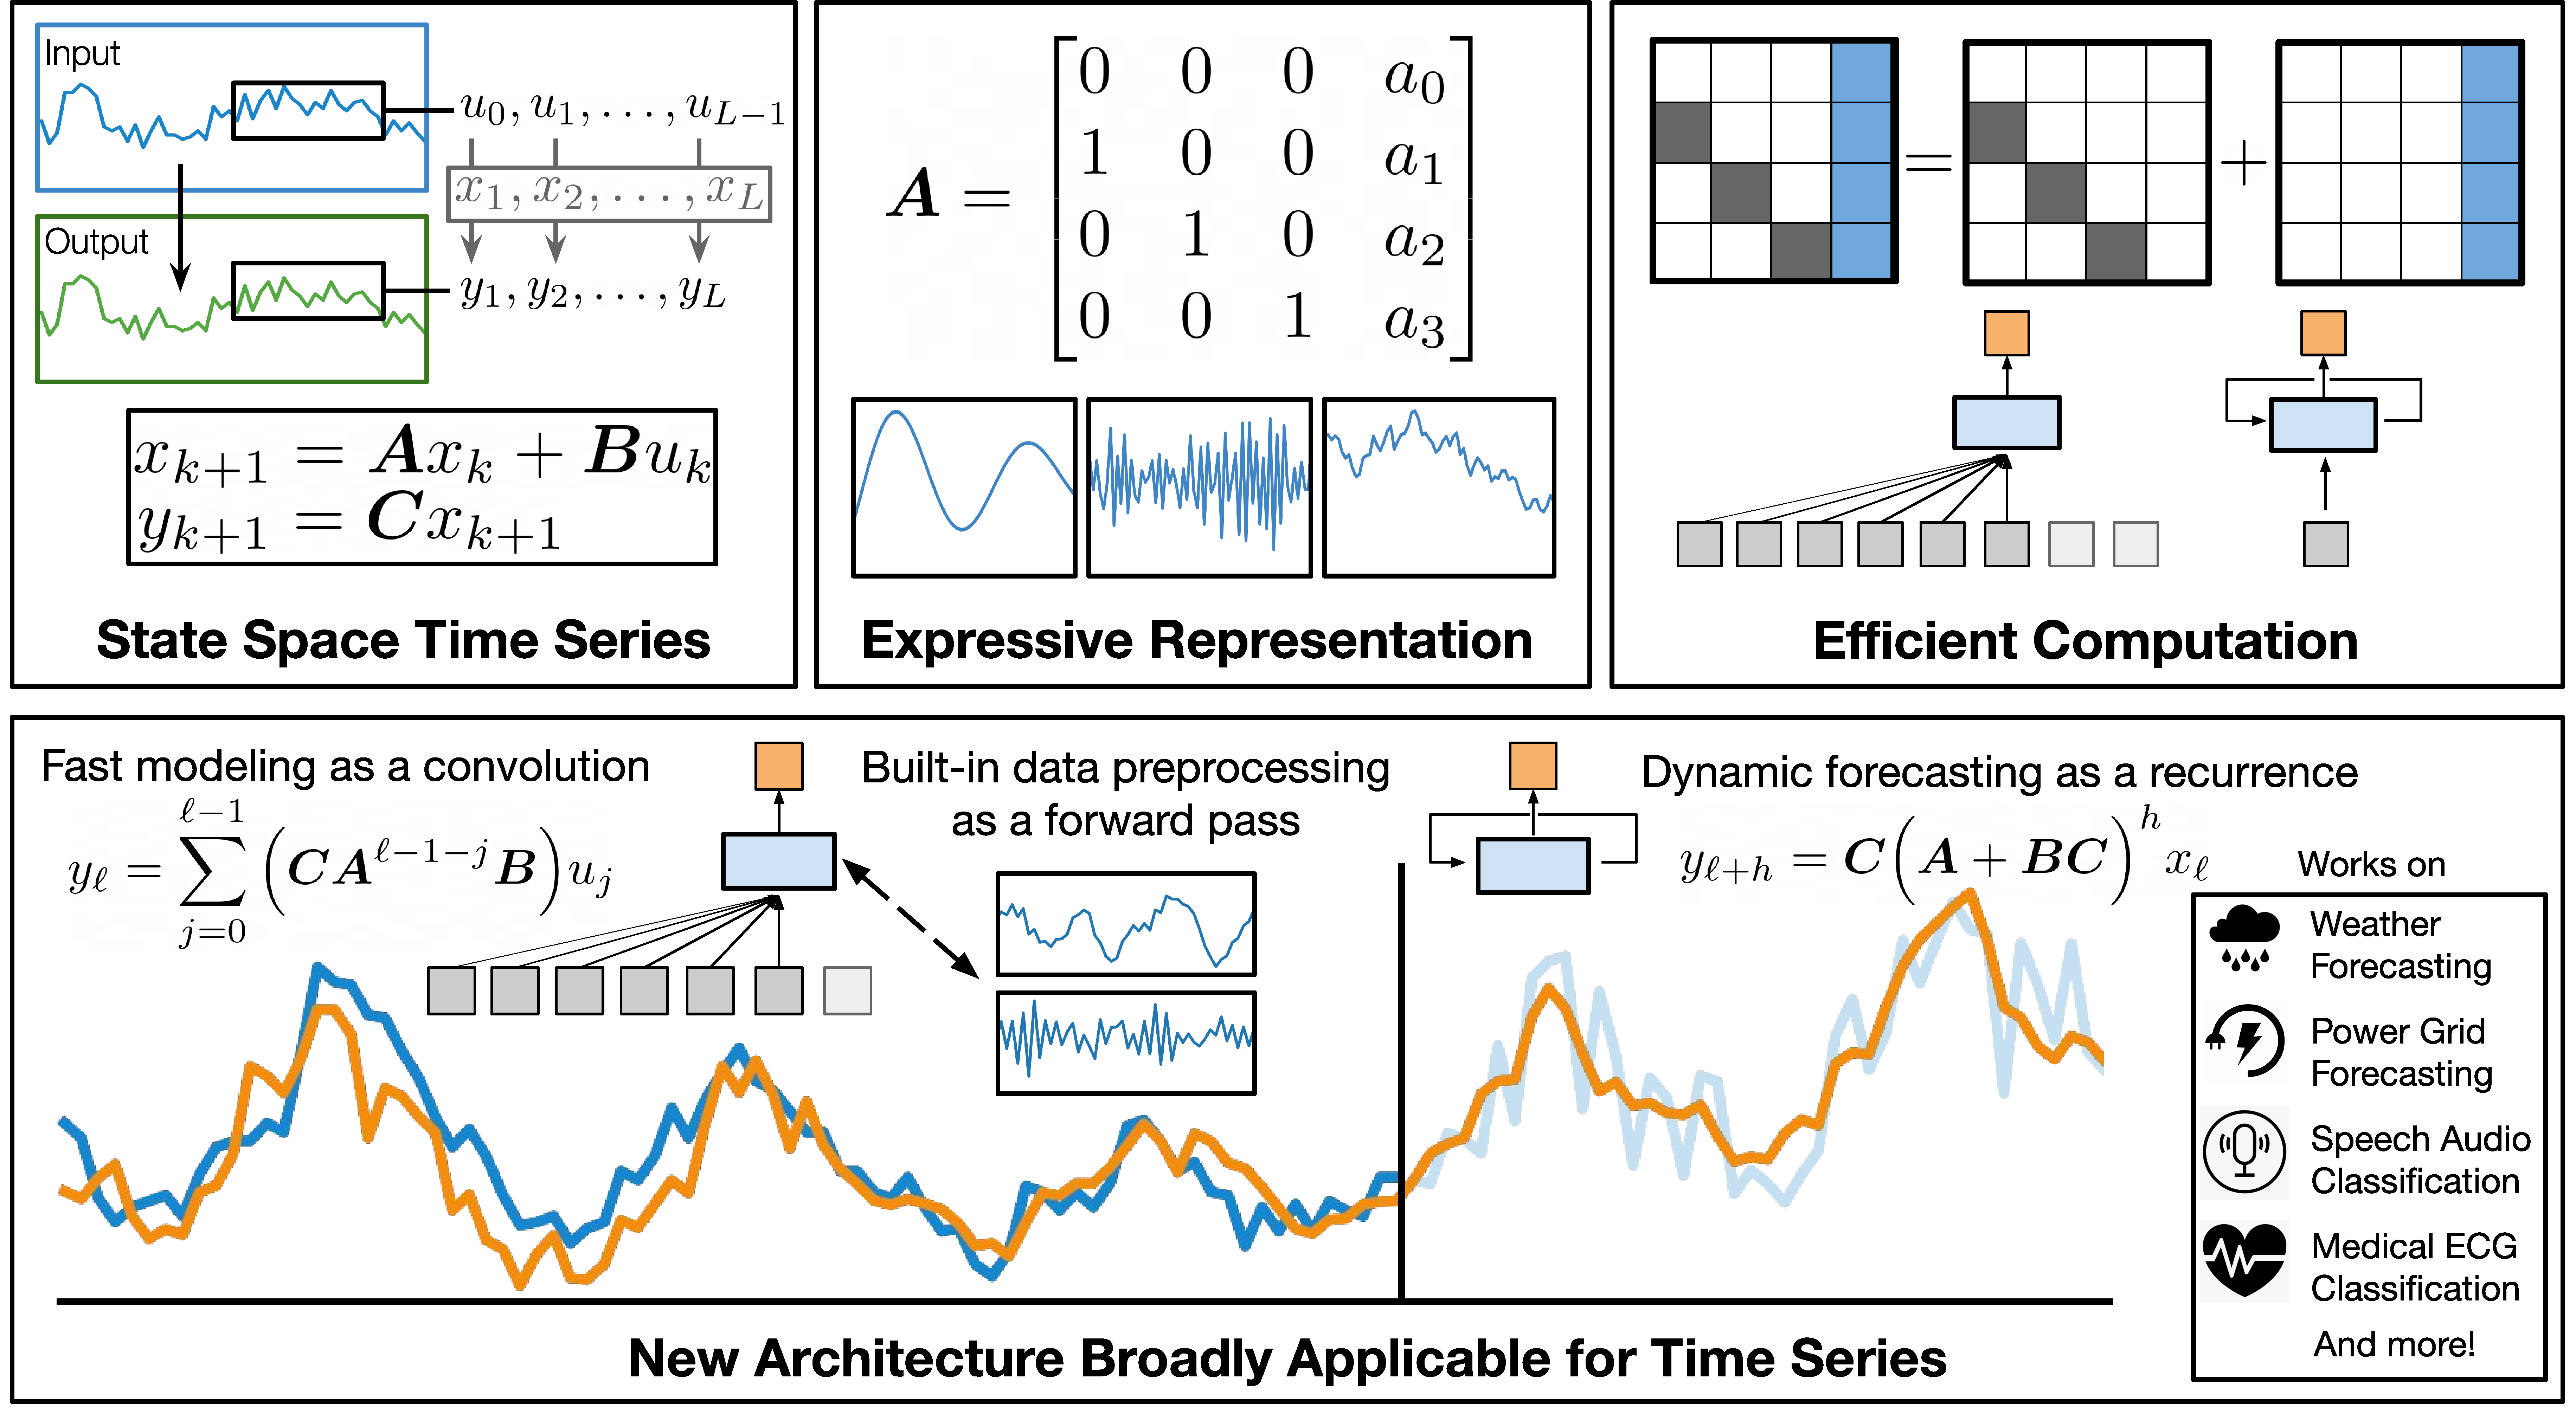
\includegraphics[width=1\textwidth]{_ICLR2023_paper/figures/time_series_ssm_use_this_2_levels_refactor1.pdf}
 \caption{We learn time series processes as state-space models (SSMs) (\textbf{top left}). We represent SSMs with the \textit{companion matrix}, which is a highly expressive representation for discrete time series  (\textbf{top middle}), and compute such SSMs efficiently as convolutions or recurrences via a shift + low-rank decomposition (\textbf{top right}). We use these SSMs to build \ourmethod{}, a new time series architecture broadly effective across tasks and domains (\textbf{bottom}).}
  \label{fig:overvew_fig1}
\end{figure}

% Our Method
%
% We thus propose \textbf{\ourmethod{}}, a new deep learning time series architecture. 
%
% Towards more effective time series modeling, 



We thus propose \textbf{\textsc{SpaceTime}}, a deep state-\textbf{space} architecture for effective \textbf{time} series modeling. 
% For more accurate forecasting and classification, 
To achieve this,
we focus on improving each criteria via three core contributions:

% \begin{enumerate}[itemsep=0.1pt,topsep=0pt,leftmargin=*]
\begin{enumerate}[topsep=0pt,leftmargin=*]
    \item For expressivity, our key idea and building block is a linear layer that models time series processes as \emph{state-space models} (SSMs) via the \emph{companion matrix} (Fig.~\ref{fig:overvew_fig1}). 
    We start with SSMs due to their connections to both classical time series analysis~\citep{kalman1960new, hamilton1994state} and recent deep learning advances~\citep{gu2021efficiently}. Classically, many time series models such as ARIMA and exponential smoothing (ETS) can be expressed as SSMs~\citep{box1970time, winters1960forecasting}. 
    Meanwhile, recent state-of-the-art deep sequence models~\citep{gu2021efficiently} have used SSMs to outperform Transformers and LSTMs on challenging long-range benchmarks~\citep{tay2020long}.
    % Meanwhile, recent SSM-based deep learning models~\citep{gu2021efficiently} have achieved state-of-the-art sequence modeling on challenging long-range benchmarks~\citep{tay2020long}. 
    Their primary innovations show how to formulate SSMs as neural network parameters that are practical to train. However, we find limitations with these deep SSMs for time series data. While we build on their advances, we prove that these prior SSM representations~\citep{ gu2021combining, gu2021efficiently, gupta2022diagonal}
    % cite these later: rangapuram2018, salinas2020deepar, lin2021ssdnet,
    cannot capture autoregressive processes fundamental for time series. We thus specifically propose the companion matrix representation for its expressive and memory-efficient properties. 
    We prove that the companion matrix SSM recovers fundamental autoregressive (AR) and smoothing processes modeled in classical techniques such as ARIMA and ETS, while only requiring $\mathcal{O}(d)$ memory to represent an $\mathcal{O}(d^2)$ matrix. 
    Thus, \ourmethod{} inherits the benefits of prior SSM-based sequence models, while introducing improved expressivity that 
    recovers fundamental time series processes
    % apture multiple AR processes and data preprocessing techniques 
    simply through its layer weights. 
    
    \item 
    % For forecasting over long horizons, we introduce a new ``closed-loop'' view of SSMs. Previous architectures apply the SSM in an ``open-loop'' fashion \citep{gu2021efficiently}, where the output is driven by the input sequence. 
    % However, to continuously forecast to long horizons, we require that the SSM has the ability to continue forecasting the signal in the absence of an input at those time steps. 
    % Inspired by classical closed-loop control~\citep{doyle2013feedback,aastrom2021feedback}, we propose a new variant of SSMs that explicitly models the next time-step input, which enables a multi-layer \ourmethod{} network to recurrently output long horizons.
    For forecasting long horizons, we introduce a new ``closed-loop'' view of SSMs. Prior deep SSM architectures either apply the SSM as an ``open-loop'' \citep{gu2021efficiently}, where fixed-length inputs necessarily generate same-length outputs, or use closed-loop autoregression where final layer outputs are fed through the \emph{entire} network as next-time-step inputs~\citep{goel2022s}. 
    We describe issues with both approaches in Sec.~\ref{sec:forecasting_ssm}, and instead achieve autogressive forecasting in a deep network with only a single SSM layer. We do so by explicitly training the SSM layer to predict its next time-step \emph{inputs}, alongside its usual outputs. This allows the SSM to recurrently generate its own future inputs that lead to desired outputs---\ie{} those that match an observed time series---so we can forecast over many future time-steps without explicit data inputs. 
    % This allows \ourmethod{} to generate its own final-layer inputs for outputting forecasts over many future time-steps.

    \item For efficiency, we introduce an algorithm for efficient training and inference with the companion matrix SSM. We 
    % first show how the companion SSM can be computed as both a convolution and a recurrence for layer-wise forward passes and forecasting respectively.  
    exploit the companion matrix's structure as a ``shift plus low-rank'' matrix, which allows us to reduce the time and space complexity for computing SSM hidden states and outputs from $\tilde{\mathcal{O}}(d \ell )$ to $\tilde{\mathcal{O}}(d + \ell)$ in SSM state size $d$ and input sequence length $\ell$. 
\end{enumerate}
% To subsequently build a full \ourmethod{} model, we simply stack together multiple layers---which each parametrize multiple companion matrix SSMs---into  a standard encoder-decoder architecture. 

% Simply stacking these layers together into a standard encoder-decoder architecture thus builds a highly expressive and efficient time series model.

In experiments, 
% we evaluate \ourmethod{} on extensive time series forecasting and classification tasks, and test if \ourmethod{}'s contributions empirically lead to (1) expressive time series modeling, (2) long-horizon forecasting, and (3) efficient training. 
%
we find \ourmethod{} consistently obtains state-of-the-art or near-state-of-the-art results, achieving best or second-best AUROC on 6 out of 7 ECG and audio speech time series classification tasks, and best mean-squared error (MSE) on 14 out of 16 Informer benchmark forecasting tasks~\citep{zhou2021informer}. \ourmethod{} also sets a new best average ranking across \numberMonashTasks{} tasks on the Monash benchmark~\citep{godahewa2021monash}.  
% 
We connect these gains with improvements on our three effective time series modeling criteria.  %
For expressivity, on synthetic ARIMA processes \ourmethod{} learns AR processes that prior deep SSMs cannot. 
%
% via extensive synthetics. As a controlled benchmark for expressiveness, we test how well popular architectures can fit standard AR processes, and find that \ourmethod{} best learns the true time series processes via its companion matrix SSM.
% compared to prior deep SSM representations.
%via visualizations of the process's ground-truth transfer function versus those parameterized by the trained SSM weights.
%
%
For long horizon forecasting, \ourmethod{} consistently outperforms prior state-of-the-art on the longest horizons by large margins. \ourmethod{} also generalizes better to \emph{new} horizons not used for training.
%
% validate that 
% We then validate (2) by showing that trained \ourmethod{}s generalize better to new horizons that models were not trained for. We also find that on the Informer benchmark, \ourmethod{} consistently outperforms alternatives on the longest evaluation horizons by the largest margins, up to $\textbf{X}$\% relative reduction in MSE for forecasting $\textbf{Y}$ time-steps.
%
% best RMSE on 25 out of 30 tasks from the diverse Monash benchmark~\citep{godahewa2021monash}.
% setting a new record among prior classical and deep learning approaches. 
% Moreover, we find that \ourmethod{} improves forecasts to arbitrary horizons (that it was not trained on) by \%XX on the Informer benchmark. 
For efficiency, on speed benchmarks \ourmethod{} obtains 73\% and 80\% relative wall-clock speedups over parameter-matched Transformers and LSTMs respectively, when training on real-world ETTh1 data.

    \section{Methodology}
\ours follows the same framework as speculative decoding, where each decoding step primarily consists of three substeps: (1) generating candidates, (2) processing candidates, and (3) accepting candidates. For \ours, (1) is achieved by \ours heads, (2) is realized by tree attention, and since \ours heads are on top of the original model, the logits calculated in (2) can be used for substep (1) for the next decoding step. The final step (3) can be realized by either rejection sampling~\citep{leviathan2022fast,chen2023accelerating} or typical acceptance (Section~\ref{sec:typical_acceptance}). The overall pipeline is illustrated in Figure~\ref{fig:pipeline}.

In this section, we first introduce the key components of \ours, including \ours heads, and tree attention. Then, we present two levels of fine-tuning procedures for \ours to meet the needs of different use cases. Finally, we propose two extensions to \ours, including self-distillation and typical acceptance, to handle situations where no training data is available for \ours and to improve the efficiency of the decoding process, respectively.
\subsection{Key Components}
\subsubsection{\ours Heads}
\label{sec:medusa_heads}
In speculative decoding, subsequent tokens are predicted by an auxiliary draft model. This draft model must be small yet effective enough to generate continuations that the original model will accept. Fulfilling these requirements is a challenging task, and existing approaches~\citep{spector2023accelerating,miao2023specinfer} often resort to separately \emph{pre-training} a smaller model. This pre-training process demands substantial additional computational resources. For example, in \citep{miao2023specinfer}, a reported 275 NVIDIA A100 GPU hours were used. Additionally, separate pre-training can potentially create a distribution shift between the draft model and the original model, leading to continuations that the original model may not favor. \citet{chen2023accelerating} have also highlighted the complexities of serving multiple models in a distributed environment.

\textcolor{black}{To streamline and democratize the acceleration of LLM inference, we take inspiration from \citet{stern2018blockwise}, which utilizes parallel decoding for tasks such as machine translation and image super-resolution. \ours heads}
 are additional decoding heads appended to the last hidden states of the original model. Specifically, given the original model's last hidden states $h_t$ at position $t$, we add $K$ decoding heads to $h_t$. The $k$-th head is used to predict the token in the $(t+k+1)$-th position of the next tokens (the original language model head is used to predict the $(t+1)$-th position). The prediction of the $k$-th head is denoted as $p_t^{(k)}$, representing a distribution over the vocabulary, while the prediction of the original model is denoted as $p_t^{(0)}$. Following the approach of \citet{stern2018blockwise}, we utilize a single layer of feed-forward network with a residual connection for each head. We find that this simple design is sufficient to achieve satisfactory performance. The definition of the $k$-th head is outlined as:

\begin{align*}
p_t^{(k)} = \text{softmax}\left(W_2^{(k)} \cdot \left(\text{SiLU}(W_1^{(k)} \cdot h_t)+h_t\right)\right),\\
\text{where } W_2^{(k)}\in\mathbb{R}^{d\times V}, W_1^{(k)}\in\mathbb{R}^{d\times d}.
\end{align*}

\textcolor{black}{$d$ is the output dimension of the LLM's last hidden layer and $V$ is the vocabulary size.}
\textcolor{black}{We initialize $W_2^{(k)}$ identically to the original language model head, and $W_1^{(k)}$ to zero.}
This aligns the initial prediction of \ours heads with that of the original model. The SiLU activation function~\citep{elfwing2017sigmoidweighted} is employed following the Llama models~\citep{touvron2023llama}.

Unlike a draft model, \ours heads are trained in conjunction with the original backbone model, which can remain \emph{frozen} during training (\ours-1) or be trained together (\ours-2). This method allows for fine-tuning large models even on a single GPU, taking advantage of the powerful base model's learned representations. Furthermore, it ensures that the distribution of the \ours heads aligns with that of the original model, thereby mitigating the distribution shift problem. Additionally, since the new heads consist of just a single layer akin to the original language model head, \ours does not add complexity to the serving system design and is friendly to distributed settings. We will discuss the training recipe for \ours heads in Section~\ref{sec:training_recipe}.

\subsubsection{Tree Attention}
\label{sec:tree_attention}
Through \ours heads, we obtain probability predictions for the subsequent $K+1$ tokens. These predictions enable us to create length-$K+1$ continuations as candidates. While the speculative decoding studies~\citep{leviathan2022fast,chen2023accelerating} suggest sampling a single continuation as the candidate, leveraging multiple candidates during decoding can enhance the expected acceptance length within a decoding step. Nevertheless, more candidates can also raise computational demands. To strike a balance, we employ a tree-structured attention mechanism to process multiple candidates concurrently.
\begin{figure}[ht]
    \centering
    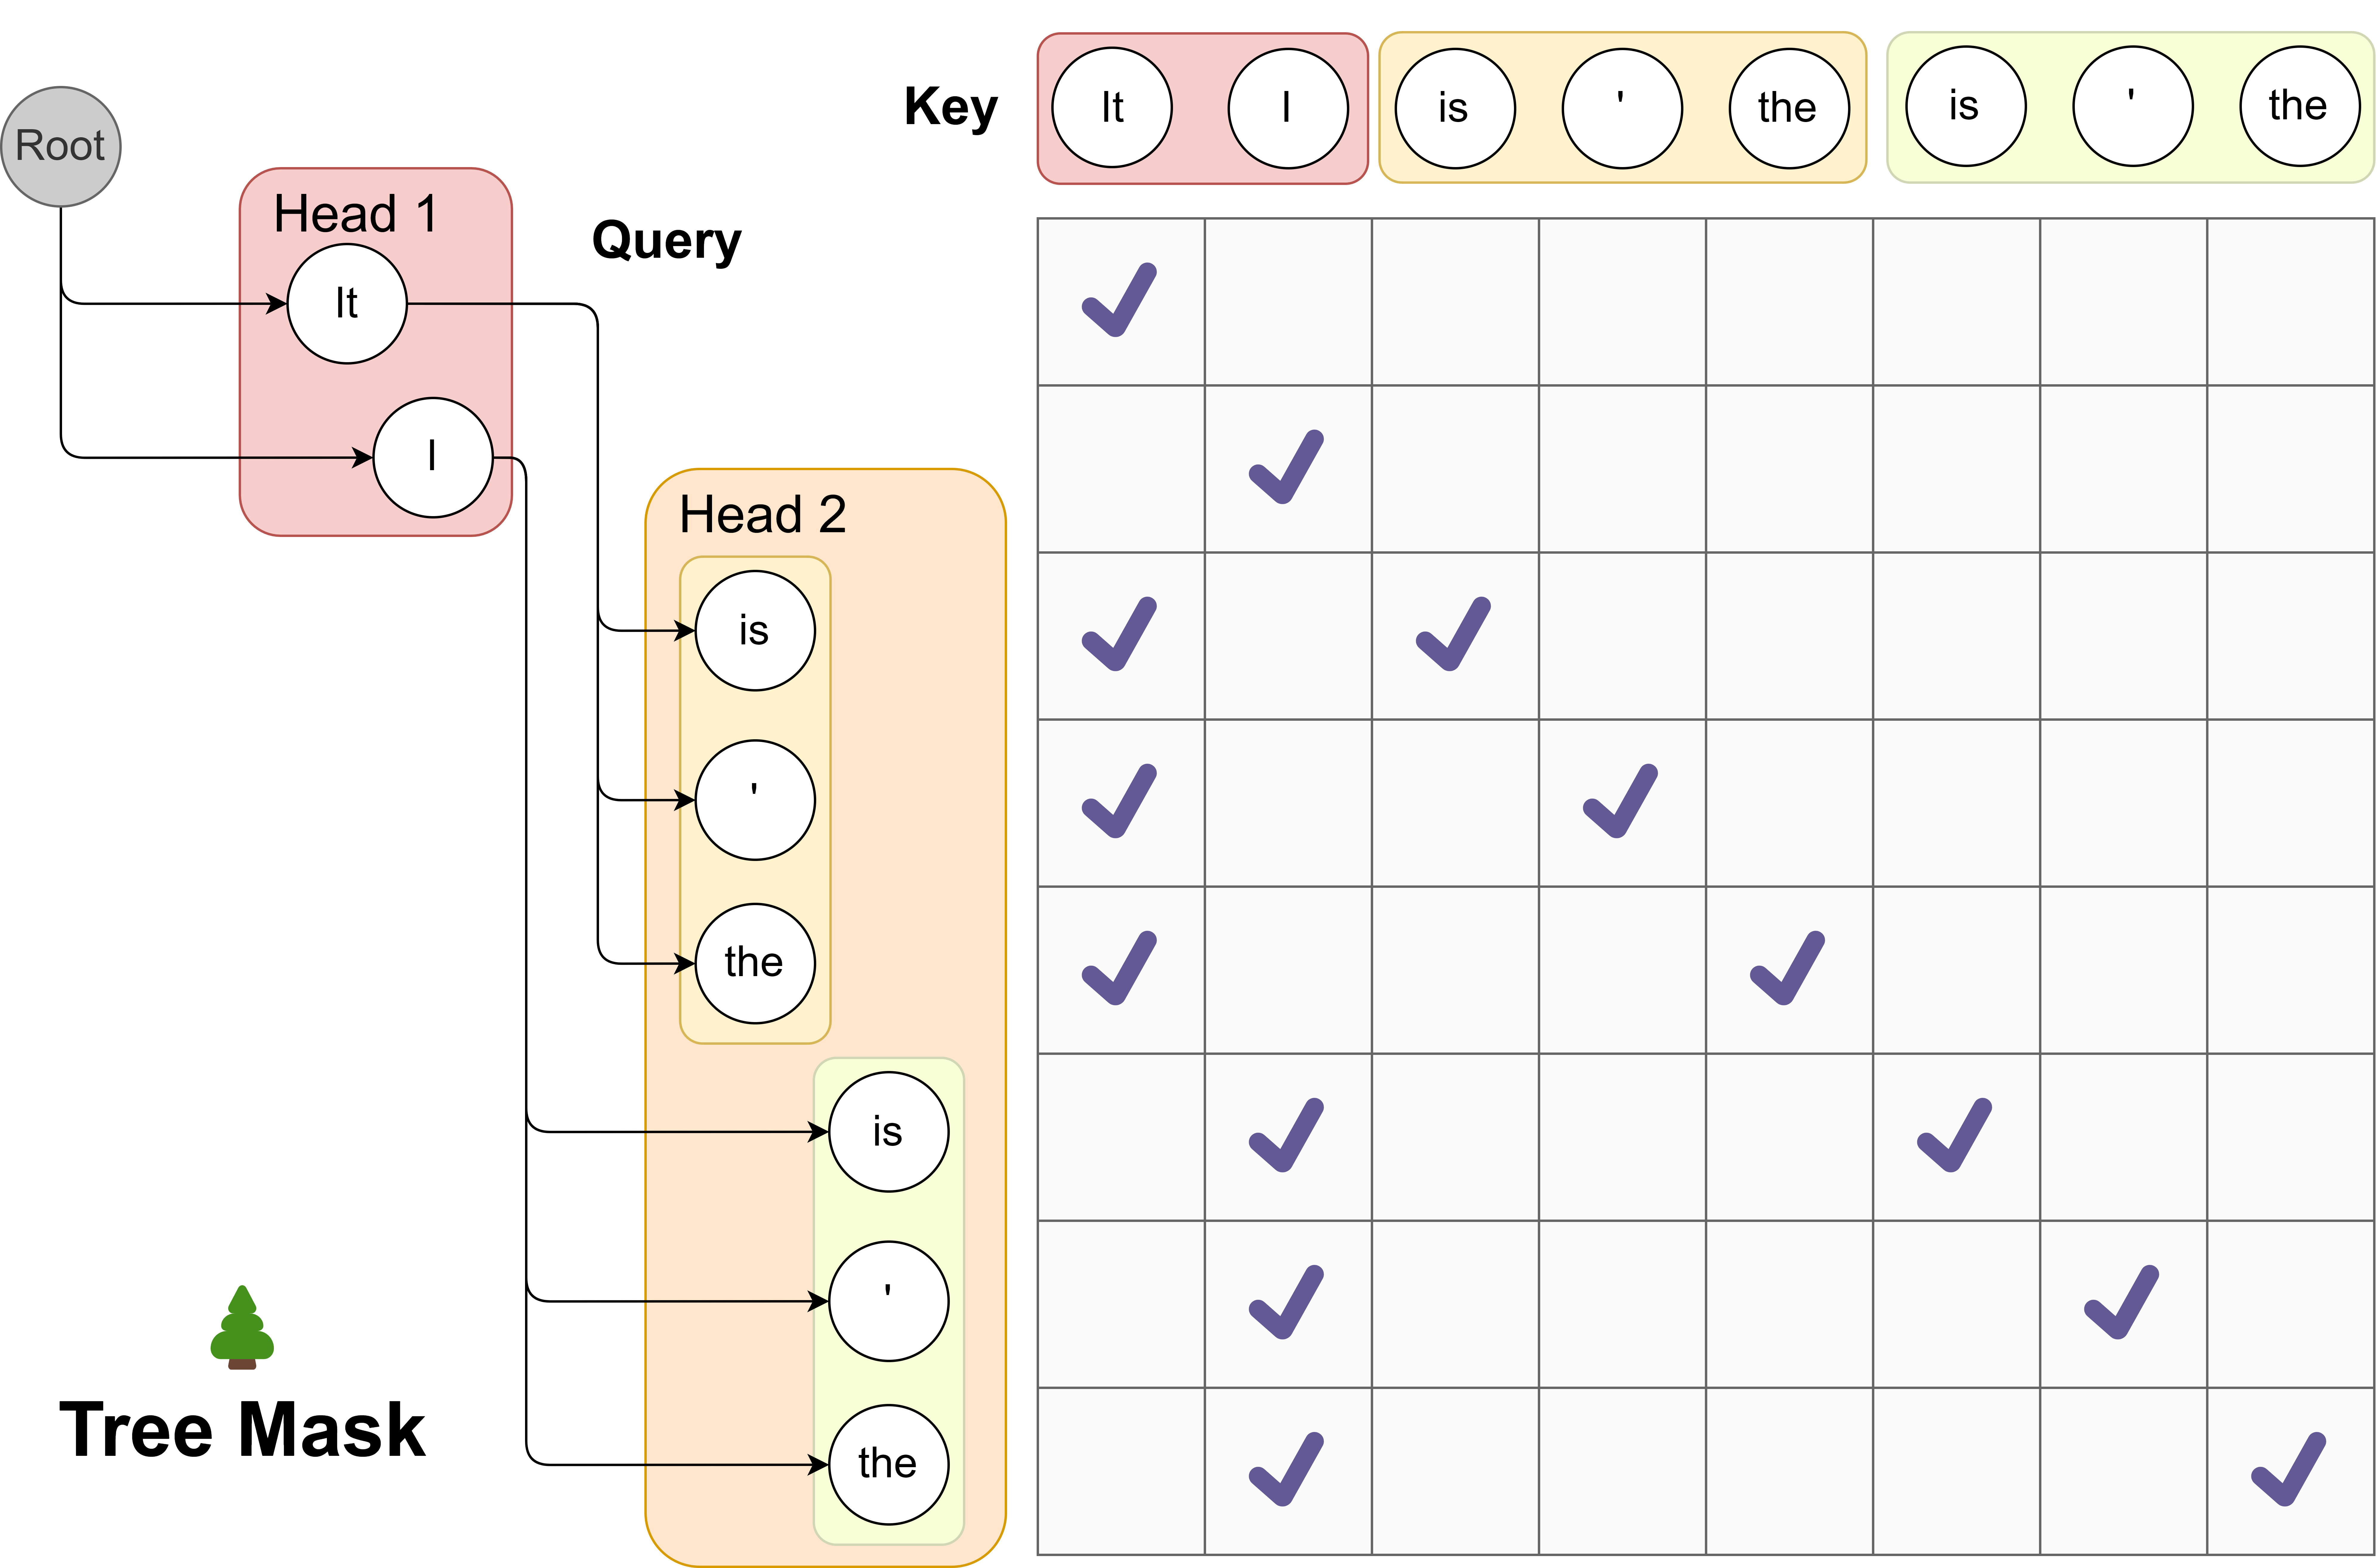
\includegraphics[width=0.45\textwidth]{tree_attention.png}
    \caption{
    We demonstrates the use of tree attention to process multiple candidates concurrently. As exemplified, the top-2 predictions from the first \ours head and the top-3 from the second result in a total of $2\times3=6$ candidates. Each of these candidates corresponds to a distinct branch within the tree structure. To guarantee that each token only accesses its predecessors, we devise an attention mask that exclusively permits attention flow from the current token back to its antecedent tokens. The positional indices for positional encoding are adjusted in line with this structure.}
    \label{fig:tree_attention}
\end{figure}
This attention mechanism diverges from the traditional causal attention paradigm. Within this framework, only tokens from the same continuation are regarded as historical data. Drawing inspiration from the concept of embedding graph structures into attention as proposed in the graph neural network domain~\citep{ying2021transformers}, we incorporate the tree structure into our attention mask, visualized in Figure~\ref{fig:tree_attention}. Remarkably, similar ideas have also been explored in independent works like \citet{miao2023specinfer,spector2023accelerating}, where they follow a bottom-up approach and construct the tree by merging multiple candidates generated by a draft model. In our method, we instead take a top-down approach to build the tree thanks to the structure of candidates generated by \ours heads. For a given $k$-th head, its top-$s_k$ predictions serve as the basis for candidate formation, where $s_k$ is a designated hyperparameter. These candidates are established by determining the Cartesian product of the top-$s_k$ predictions from each head. For instance, in Figure~\ref{fig:tree_attention}, with $s_1=2$ and $s_2=3$, each first head prediction can be succeeded by any prediction from the second head. This leads to a tree structure where $s_k$ branches exist at the $k$-th level (considering a virtual root as the $0$-level, in practice, this $0$-level is for the prediction of the language model head of the original model, which can be sampled independently). Within this tree, only a token's predecessors are seen as historical context, and our attention mask ensures that the attention is only applied on a token's predecessors. By employing this mask and properly setting the positional indices for positional encoding, we can process numerous candidates simultaneously without the need to expand the batch size. The cumulative number of new tokens is calculated as $\sum_{k=1}^K \prod_{i=1}^k s_i$.

In this section, we demonstrate the most simple and regular way to construct the tree structure by taking the Cartesian product. However, it is possible to construct the tree structure in a more sophisticated way and exploit the unbalanced accuracy of different top predictions of different heads. We will discuss this in Section~\ref{sec:optimized_tree_construction}.
\subsection{Training Strategies}
\label{sec:training_recipe}
At the most basic level, we can train \ours heads by freezing the backbone model and fine-tuning \ours heads. However, training the backbone in conjunction with the \ours heads can significantly enhance the accuracy of the \ours heads. Depending on the computational resources and the specific reqirements of the use case, we propose two levels of training strategies for \ours heads.

In this section, we assume the availability of a training dataset that aligns with the target model’s output distribution. This could be the dataset used for Supervised Fine-Tuning (SFT) of the target model. We will discuss eliminating the need for such a dataset using a self-distillation approach in Section~\ref{sec:self_distillation}.
\subsubsection{\ours-1: Frozen Backbone}
\label{sec:frozen_backbone}
To train \ours heads with a frozen backbone model, we can use the cross-entropy loss between the prediction of \ours heads and the ground truth. Specifically, given the ground truth token $y_{t+k+1}$ at position $t+k+1$, the loss for the $k$-th head is $\mathcal{L}_k = -\log p_t^{(k)}(y_{t+k+1})$ where $p_t^{(k)}(y)$ denotes the probability of token $y$ predicted by the $k$-th head. We also observe that $\mathcal{L}_k$ is larger when $k$ is larger, which is reasonable since the prediction of the $k$-th head is more uncertain when $k$ is larger. Therefore, we can add a weight $\lambda_k$ to $\mathcal{L}_k$ to balance the loss of different heads. And the total \ours loss is:
\begin{align}
    \label{eq:loss_medusa_1}
    \mathcal{L}_{\text{\ours-1}} = \sum_{k=1}^K -\lambda_k\log p_t^{(k)}(y_{t+k+1}).
\end{align}

In practice, we set $\lambda_k$ as the $k$-th power of a constant like $0.8$. Since we only use the backbone model for providing the hidden states, we can use a quantized version of the backbone model to reduce the memory consumption. This introduces a more democratized way to accelerate LLM inference, as with the quantization, \ours can be trained for a large model on a single consumer GPU similar to QLoRA~\citep{dettmers2023qlora}. The training only takes a few hours (e.g., 5 hours for \ours-1 on Vicuna 7B model with a single NVIDIA A100 PCIE GPU to train on 60k ShareGPT samples).
\subsubsection{\ours-2: Joint Training}
\label{sec:joint_training}
To further improve the accuracy of \ours heads, we can train \ours heads together with the backbone model. However, this requires a special training recipe to preserve the backbone model's next-token prediction capability and output quality. To achieve this, we propose three strategies:
\begin{itemize}
    \item \textbf{Combined loss}: To keep the backbone model's next-token prediction capability, we need to add the cross-entropy loss of the backbone model $\mathcal{L}_{\text{LM}}=-\log p_t^{(0)}(y_{t+1})$ to the \ours loss. We also add a weight $\lambda_0$ to balance the loss of the backbone model and the \ours heads. Therefore, the total loss is:
    \begin{align}
        \label{eq:loss_medusa_2}
        \mathcal{L}_{\text{\ours-2}} = \mathcal{L}_{\text{LM}} + \lambda_0\mathcal{L}_{\text{\ours-1}}.
    \end{align}
    \item \textbf{Differential learning rates}: Since the backbone model is already well-trained and the \ours heads need more training, we can use separate learning rates for them to enable faster convergence of \ours heads while preserving the backbone model's capability.
    \item \textbf{Heads warmup}: Noticing that at the beginning of training, the \ours heads have a large loss, which leads to a large gradient and may distort the backbone model's parameters. Following the idea from \citet{kumar2022finetuning}, we can employ a two-stage training process. In the first stage, we only train the \ours heads as \ours-1. In the second stage, we train the backbone model and \ours heads together with a warmup strategy. Specifically, we first train the backbone model for a few epochs, then train the \ours heads together with the backbone model. Besides this simple strategy, we can also use a more sophisticated warmup strategy by gradually increasing the weight $\lambda_0$ of the backbone model's loss. We find both strategies work well in practice.
\end{itemize}
Putting these strategies together, we can train \ours heads together with the backbone model without hurting the backbone model's capability. Moreover, this recipe can be applied together with Supervised Fine-Tuning (SFT), enabling us to get a model with native \ours support.
\subsubsection{How to Select the Number of Heads}
Empirically, we found that five heads are sufficient at most. Therefore, we recommend training with five heads and referring to the strategy described in Section~\ref{sec:optimized_tree_construction} to determine the optimal configuration of the tree attention. With optimized tree attention, sometimes three or four heads may be enough for inference. In this case, we can ignore the redundant heads without overhead.

\subsection{Extensions}
\subsubsection{Typical Acceptance}
\label{sec:typical_acceptance}
In speculative decoding papers~\citep{leviathan2022fast,chen2023accelerating}, authors employ rejection sampling to yield diverse outputs that align with the distribution of the original model. However, subsequent implementations~\citep{gante2023assisted,spector2023accelerating} reveal that this sampling strategy results in diminished efficiency as the sampling temperature increases. Intuitively, this can be comprehended in the extreme instance where the draft model is the same as the original one\textcolor{black}{:} 
Using greedy decoding, all output of the draft model will be accepted, therefore maximizing the efficiency. 
Conversely, rejection sampling introduces extra overhead, as the draft model and the original model are sampled independently. Even if their distributions align perfectly, the output of the draft model may still be rejected.

However, in real-world scenarios, sampling from language models is often employed to generate diverse responses, and the temperature parameter is used merely to modulate the ``creativity'' of the response. Therefore, higher temperatures should result in more opportunities for the original model to accept the draft model's output. We ascertain that it is typically unnecessary to match the distribution of the original model. Thus, we propose employing a \emph{typical acceptance} scheme to select plausible candidates rather than using rejection sampling. This approach draws inspiration from truncation sampling studies~\citep{hewitt2022truncation} (refer to \textcolor{black}{Appendix}~\ref{sec:related_work} for an in-depth explanation). Our objective is to choose candidates that are \emph{typical}, meaning they are not exceedingly improbable to be produced by the original model. We use the prediction probability from the \emph{original model} as a natural gauge for this and establish a threshold based on the prediction distribution to determine acceptance. Specifically, given $x_1, x_2, \cdots, x_n$ as context, when evaluating the candidate sequence \textcolor{black}{$(x_{n+1}, x_{n+2}, \cdots, x_{n+K+1})$ }(composed by top predictions of the original language model head and \ours heads), we consider the condition
\begin{align*}
p_{\text{original}}(x_{n+k}|x_1, x_2, \cdots, x_{n+k-1}) > \\\min\rbr{\epsilon, \delta\exp\rbr{-H(p_{\text{original}}(\cdot|x_1, x_2, \cdots, x_{n+k-1}))}},
\end{align*}
where $H(\cdot)$ denotes the entropy function, and $\epsilon, \delta$ are \textcolor{black}{the hard threshold and the entropy-dependent
threshold respectively}. This criterion is adapted from \citet{hewitt2022truncation} and rests on two observations: (1) tokens with relatively high probability are meaningful, and (2) when the distribution's entropy is high, various continuations may be deemed reasonable. During decoding, every candidate is evaluated using this criterion, and a \emph{prefix} of the candidate is accepted if it satisfies the condition. To guarantee the generation of at least one token at each step, we apply \emph{greedy decoding} for the first token and \emph{unconditionally} accept it while employing typical acceptance for subsequent tokens. The final prediction for the current step is determined by the \emph{longest accepted prefix} among all candidates.

Examining this scheme leads to several insights. Firstly, when the temperature is set to $0$, it reverts to greedy decoding, as only the most probable token possesses non-zero probability. As the temperature surpasses $0$, the outcome of greedy decoding will consistently be accepted with appropriate $\epsilon, \delta$, since those tokens have the maximum probability, yielding maximal speedup. Likewise, in general scenarios, an increased temperature will correspondingly result in longer accepted sequences, as corroborated by our experimental findings.

Empirically, we verify that typical acceptance can achieve a better speedup while maintaining a similar \textcolor{black}{generation quality} as shown in Figure~\ref{fig:threshold_ablation}.
\subsubsection{Self-Distillation}
\label{sec:self_distillation}
In Section~\ref{sec:training_recipe}, we assume the existence of a training dataset that matches the target model's output distribution. However, this is not always the case. For example, the model owners may only release the model without the training data, or the model may have gone through a Reinforcement Learning with Human Feedback (RLHF) procedure, which makes the output distribution of the model different from the training dataset. To tackle this issue, we propose an automated self-distillation pipeline to use the model itself to generate the training dataset for \ours heads, which matches the output distribution of the model.

The dataset generation process is straightforward. We first take a public seed dataset from a domain similar to the target model; for example, using the ShareGPT~\citep{sharegpt2023} dataset for chat models. Then, we simply take the prompts from the dataset and ask the model to reply to the prompts. In order to obtain multi-turn conversation samples, we can sequentially feed the prompts from the seed dataset to the model. Or, for models like Zephyr 7B~\citep{tunstall2023zephyr}, which are trained on both roles of the conversation, they have the ability to self-talk, and we can simply feed the first prompt and let the model generate multiple rounds of conversation.

For \ours-1, this dataset is sufficient for training \ours heads. However, for \ours-2, we observe that solely using this dataset for training the backbone and \ours heads usually leads to a lower generation quality. In fact, even without training \ours heads, training the backbone model with this dataset will lead to performance degradation. This suggests that we also need to use the original model's probability prediction instead of using the ground truth token as the label for the backbone model, similar to classic knowledge distillation works~\citep{kim2016sequencelevel}. Concretely, the loss for the backbone model is:
\begin{align*}
    \mathcal{L}_{\text{LM-distill}} = KL(p_{\text{original},t}^{(0)}||p_t^{(0)}),
\end{align*}
where $p_{\text{original},t}^{(0)}$ denotes the probability distribution of the original model's prediction at position $t$.

However, naively, to obtain the original model's probability prediction, we need to maintain two models during training, increasing the memory requirements. To further alleviate this issue, we propose a simple yet effective way to exploit the self-distillation setup. We can use a parameter-efficient adapter like LoRA~\citep{hu2021lora} for fine-tuning the backbone model. In this way, the original model is simply the model with the adapter turned off. Therefore, the distillation does not require additional memory consumption. Together, this self-distillation pipeline can be used to train \ours-2 without hurting the backbone model's capability and introduce almost no additional memory consumption. Lastly, one tip about using self-distillation is that it is preferable to use LoRA without quantization in this case, otherwise, the teacher model will be the quantized model, which may lead to a lower generation quality.

\subsubsection{Searching for the Optimized Tree Construction}
\label{sec:optimized_tree_construction}
In Section~\ref{sec:tree_attention}, we present the simplest way to construct the tree structure by taking the Cartesian product. However, with a fixed budget for the number of total nodes in the tree, a regular tree structure may not be the best choice. Intuitively, those candidates composed of the top predictions of different heads may have different accuracies. Therefore, we can leverage an estimation of the accuracy to construct the tree structure.

Specifically, we can use a calibration dataset and calculate the accuracies of the top predictions of different heads. Let $a_k^{(i)}$ denote the accuracy of the $i$-th top prediction of the $k$-th head\footnote{Here, the accuracy is defined for the single top $i$-th token, i.e., this accuracy is equal to top-$i$ accuracy minus top-$(i-1)$ accuracy.}. Assuming the accuracies are independent, we can estimate the accuracy of a candidate sequence composed by the top $\sbr{i_1, i_2, \cdots, i_k}$ predictions of different heads as $\prod_{j=1}^k a_j^{(i_j)}$. Let $I$ denote the set of all possible combinations of $\sbr{i_1, i_2, \cdots, i_k}$ and each element of $I$ can be mapped to a node of the tree (not only leaf nodes but all nodes are included). Then, the expectation of the acceptance length of a candidate sequence is:
\begin{align*}
    \sum_{\sbr{i_1, i_2, \cdots, i_k}\in I}\prod_{j=1}^k a_j^{(i_j)}.
\end{align*}
Thinking about building a tree by adding nodes one by one, the contribution of a new node to the expectation is exactly the accuracy associated with the node. Therefore, we can greedily add nodes to the tree by choosing the node that is connected to the current tree and has the highest accuracy. This process can be repeated until the total number of nodes reaches the desired number. In this way, we can construct a tree that maximizes the expectation of the acceptance length. Further details can be found in Appendix~\ref{appendix:sparse_tree}.


    \vspace{-0.2cm}
\section{Experiments Details}
\label{sec:exp}

\vspace{-0.2cm}
\subsection{Roadmap Insights on FFHQ-256\texorpdfstring{~\cite{sg1}}{}}
\label{sub:arc-experiments}
\vspace{-0.1cm}
As per Table~\ref{tab:roadmap}, Config A (vanilla StyleGAN2) achieves an FID of 7.52 using the official implementation on FFHQ-256. Config B with all tricks removed achieves an FID of 12.46---performance drops as expected. 
Config C, with a well-behaved loss, achieves an FID of 11.65. But, now training is sufficiently stable to improve the architecture.

Config D, which improves $G$ and $D$ based on the classic ResNet and ConvNeXt findings, achieves an FID of 9.95. The output skips of the StyleGAN2 generator are no longer useful given our new architecture; including them produces a worse FID of 10.17. Karras~\etal find that the benefit of output skips is mostly related to gradient magnitude dynamics~\cite{sg3}, and this has been addressed by our ResNet architecture. For StyleGAN2, Karras~\etal conclude that a ResNet architecture is harmful to $G$~\cite{sg2}, but this is not true in our case as their ResNet implementation is considerably different from ours: 1) Karras~\etal use one 3-3 residual block for each resolution stage, while we have a separate transition layer and two 1-3-1 residual blocks; 2) i.3) and i.4) are violated as they do not have a linear residual block~\cite{mobnet} and the transition layer is placed on the skip branch of the residual block rather than the stem; 3) the essential principle of ResNet~\cite{resnet}---identity mapping~\cite{resnet2}---is violated as Karras~\etal divide the output of the residual block by $\sqrt{2}$ to avoid variance explosion due to the absence of a proper initialization scheme.

For Config E, we conduct two experiments that ablate i.\ref{item:i1} (increased width with depthwise conv.) and i.\ref{item:i2} (an inverted bottleneck). We add GroupedConv and reduce the bottleneck compression ratio to two given the same model size. Each bottleneck is now 1.5$\times$ the width of Config A, and the FID drops to 7.51, surpassing the performance of StyleGAN2. By inverting the stem and the bottleneck dimensions to enhance the capacity of GroupedConv, our final model achieves an FID of 7.05, exceeding StyleGAN2.


\begin{wraptable}[12]{r}{6.5cm}
\vspace{-1.25cm}
\centering
\caption{StackedMNIST 1000-mode coverage.}
% Our model outperforms other GANs in terms of $D_\text{KL}$, indicating that we are better able to recover the distribution.}
\vspace{-0.4cm}
\resizebox{0.8\linewidth}{!}{
\begin{tblr}{
  cell{2}{2} = {c},
  cell{2}{3} = {c},
  cell{3}{2} = {c},
  cell{3}{3} = {c},
  cell{4}{2} = {c},
  cell{4}{3} = {c},
  cell{5}{2} = {c},
  cell{5}{3} = {c},
  cell{6}{2} = {c},
  cell{6}{3} = {c},
  cell{7}{2} = {c},
  cell{7}{3} = {c},
  cell{8}{2} = {c},
  cell{8}{3} = {c},
  cell{9}{2} = {c},
  cell{9}{3} = {c},
  cell{10}{2} = {c},
  cell{10}{3} = {c},
  cell{11}{2} = {c},
  cell{11}{3} = {c},
  cell{12}{2} = {c},
  cell{12}{3} = {c},
  hline{2,12} = {1-3}{},
}
Model     & \# modes$\uparrow$ & $D_\text{KL}$$\downarrow$            &  \\
DCGAN~\cite{dcgan}     & 99            & 3.40\phantom{0}&  \\
VEEGAN~\cite{srivastava2017veegan}    & 150           & 2.95\phantom{0}&  \\
WGAN-GP~\cite{wgan-gp}& 959           & 0.73\phantom{0}&  \\
PacGAN~\cite{pacgan}    & 992           & 0.28\phantom{0}&  \\
StyleGAN2~\cite{sg2} & 940           & 0.42\phantom{0}&  \\
PresGAN~\cite{presgan}   & \textbf{1000} & 0.12\phantom{0}&  \\
Adv. DSM~\cite{advsm}  & \textbf{1000} & 1.49\phantom{0}&  \\
VAEBM~\cite{vaebm}     & \textbf{1000} & 0.087          &  \\
DDGAN~\cite{ddgan}     & \textbf{1000} & 0.071          &  \\
MEG~\cite{meg}       & \textbf{1000} & 0.031          &  \\
Ours---Config E     & \textbf{1000} & \textbf{0.029} &  
\end{tblr}
}
\label{tab:stackedmnist}
\end{wraptable}%

\subsection{Mode Recovery --- StackedMNIST\texorpdfstring{~\cite{metz2016unrolled}}{}} 
\vspace{-0.1cm}
We repeat the earlier experiment in 1000-mode convergence on StackedMNIST (unconditional generation), but this time with our updated architecture and with comparisons to SOTA GANs and likelihood-based methods (Tab.~\ref{tab:stackedmnist}, Fig.~\ref{fig:stacked-mnist}). 
One advantage brought up of likelihood-based models such as diffusion over GANs is that they achieve mode coverage~\cite{adm}. We find that most GANs struggle to find all modes. But, PresGAN~\cite{presgan}, DDGAN~\cite{ddgan}, and our approach are successful. Further, our method outperforms all other tested GAN models in term of KL divergence.

\subsection{FID --- FFHQ-256\texorpdfstring{~\cite{sg1}}{} (Optimized)}
\vspace{-0.1cm}
We train Config E model until convergence and with optimized hyperparameters and training schedule on FFHQ at 256$\times$256 (unconditional generation) (Tab.~\ref{tab:ffhq256}, Figs.~\ref{fig:ffhq-256-teaser} and~\ref{fig:ffhq-256}). 
Please see our supplemental material for training details.
%The hyperparameters and schedule are listed in the supplemental material. 
Our model outperforms existing StyleGAN methods, plus four more recent diffusion-based methods. On this common dataset experimental setting, many methods (not listed here) use the bCR~\cite{zhao2021improved} trick---this has only been shown to improve performance on FFHQ-256 (not even at different resolutions of FFHQ)~\cite{zhao2021improved, zhang2022styleswin}. We do not use this trick. 
% no such tricks in our method.
% JT Try to minimize embellishment...
% This is particularly impressive given the fact that the dataset FFHQ was designed for StyleGAN~\cite{sg1} and the StyleGAN series of models were optimized with this specific dataset in mind.
% to achieve this performance.

\subsection{FID --- FFHQ-64\texorpdfstring{~\cite{edm}}{}}
\vspace{-0.1cm}
To compare with EDM~\cite{edm} directly, we evaluate our model on FFHQ at 64$\times$64 resolution. For this, we remove the two highest resolution stages of our 256$\times$256 model, resulting in a generator that is less than half the number of parameters as EDM. Despite this, our model outperforms EDM on this dataset and needs one function evaluation only (Tab.~\ref{tab:ffhq64}).

\begin{figure}
\begin{floatrow}
    %\hspace{-0.75cm}%
    \capbtabbox{%
        \centering
        \resizebox{\linewidth}{!}{
        \begin{tblr}{
          column{2,3} = {r},
          cell{1}{2} = {c},
          cell{1}{3} = {c},
          hline{2,5,9,10} = {-}{},
        }
        Model       & NFE$\downarrow$ & FID$\downarrow$  \\
        StyleGAN2~\cite{sg2}   & 1               & 3.78 \\
        StyleGAN3-T~\cite{sg3} & 1               & 4.81 \\
        StyleGAN3-R~\cite{sg3} & 1               & 3.92 \\
        LDM~\cite{rombach2022high} & 200               & 4.98\\
        ADM (DDIM)~\cite{adm,compdiff} & 500               & 8.41\\
        ADM (DPM-Solver)~\cite{adm,compdiff} & 500               & 8.40\\
        Diffusion Autoencoder~\cite{diffae,compdiff} & 500               & 5.81\\
        Ours---Config E  & 1               & 2.75 \\
        \emph{With ImageNet feature leakage~\cite{kynkaanniemi2022role}:} & & \\
        PolyINR*~\cite{singh2023polynomial} & 1               & 2.72 \\
        StyleGAN-XL*~\cite{sgxl} & 1               & 2.19 \\
        StyleSAN-XL*~\cite{takida2024san} & 1               & 1.68 \\
        \end{tblr}
        }
    }{%
        \caption{
        \label{tab:ffhq256}FFHQ-256. * denotes models that leak ImageNet features.}
    }
    %
    \capbtabbox{%
        \centering
        \resizebox{0.85\linewidth}{!}{
        \begin{tblr}{
          column{2} = {r},
          column{3} = {r},
          hline{2,5,8} = {-}{},
        }
        Model         & NFE$\downarrow$ & FID$\downarrow$ \\
        StyleGAN2~\cite{sg2,anycostgan}     & 1               & 3.32            \\
        MSG-GAN~\cite{karnewar2020msg,anycostgan}       & 1               & 2.7             \\
        Anycost GAN~\cite{anycostgan}   & 1               & 2.52            \\
        VE~\cite{sde,edm}            & 79              & 25.95           \\
        VP~\cite{sde,edm}            & 79              & 3.39            \\
        EDM~\cite{edm}           & 79              & 2.39            \\
        Ours—Config E & 1               & 1.95 \\
        \end{tblr}
        }
    }{%
        \caption{\label{tab:ffhq64}FFHQ-64.}
    }
\end{floatrow}
\vspace{-0.25cm}
\end{figure}


% \begin{figure}
% \begin{floatrow}
%     \capbtabbox{%
%         \centering
%         \resizebox{0.8\linewidth}{!}{
%         \begin{tblr}{
%           column{2,3} = {r},
%           cell{1}{2} = {c},
%           cell{1}{3} = {c},
%           hline{2,9,13} = {-}{},
%         }
%         Model               & NFE$\downarrow$ & FID$\downarrow$ \\
%         BigGAN~\cite{biggan}              & 1               & 14.73 \\
%         TransGAN~\cite{trans}            & 1               & 9.26 \\
%         ViTGAN~\cite{vitgan}              & 1               & 6.66 \\
%         DDGAN~\cite{ddgan}               & 4               & 3.75 \\
%         Diffusion StyleGAN2~\cite{diffusiongan} & 1               & 3.19 \\
%         StyleGAN2 + ADA~\cite{sg2ada}     & 1               & 2.42 \\
%         StyleGAN3-R + ADA~\cite{sg3,studio}   & 1               & 10.83 \\
%         DDPM~\cite{ddpm}               & 1000            & 3.21 \\
%         DDIM~\cite{ddim}                & 50             & 4.67 \\
%         VE~\cite{sde,edm}                  & 35              & 3.11 \\
%         VP~\cite{sde,edm}                  & 35              & 2.48 \\
%         Ours---Config E     & 1               & 1.96 \\
%         \hline
%         \emph{With ImageNet feature leakage~\cite{kynkaanniemi2022role}:} & & \\
%         StyleGAN-XL*~\cite{sgxl}       & 1               & 1.85 \\
%         \end{tblr}
%         }
%     }{%
%         \caption{\label{tab:cifar10}CIFAR-10.}
%     }
%         % \begin{tblr}{
%         %   column{2,3} = {r},
%         %   cell{1}{2}{3} = {},
%         %   hline{2,9,13} = {-}{},
%         % }
%         % Model               & FID$\downarrow$ & Params          \\
%         % BigGAN~\cite{biggan}              & 14.73  & --       \\
%         % TransGAN~\cite{trans}            & 9.26 & --         \\
%         % ViTGAN~\cite{vitgan}              & 6.66 & --         \\
%         % DDGAN~\cite{ddgan}               & 3.75 & --         \\
%         % Diffusion StyleGAN2 & 3.19 & 40.1M           \\
%         % StyleGAN2 + ADA     & 2.42 & 40.1M          \\
%         % StyleGAN3-R + ADA   & 10.83 & 40.1M        \\
%         % DDPM               & 3.21 & 35.2M         \\
%         % DDIM                & 4.67 & --         \\
%         % VE~\cite{edm}                  & 3.11 & 61.8M        \\
%         % VP~\cite{edm}                  & 2.48 & 61.8M         \\
%         % Ours---Config E     & \textbf{1.99}  & 43.0M \\
%         % StyleGAN-XL*~\cite{sgxl}       & 	1.85 & 140.0M \\
%         % \end{tblr}
        
%     %     }
%     % }{%
%     %     \caption{\label{tab:cifar10}CIFAR-10.}
%     % }%
%     %\hspace{-0.75cm}%
%     %\hspace{-0.5cm}%
% \end{floatrow}
% \end{figure}

\subsection{FID --- CIFAR-10~\cite{krizhevsky2009learning}} \vspace{-0.1cm}

\begin{wraptable}[14]{r}{6.5cm}
\vspace{-0.75cm}
\centering
\caption{\label{tab:cifar10}CIFAR-10 performance.}
\vspace{-0.4cm}
\resizebox{0.9\linewidth}{!}{
    \begin{tblr}{
          column{2,3} = {r},
          cell{1}{2} = {c},
          cell{1}{3} = {c},
          hline{2,9,13} = {-}{},
        }
        Model               & NFE$\downarrow$ & FID$\downarrow$ \\
        BigGAN~\cite{biggan}              & 1               & 14.73 \\
        TransGAN~\cite{trans}            & 1               & 9.26 \\
        ViTGAN~\cite{vitgan}              & 1               & 6.66 \\
        DDGAN~\cite{ddgan}               & 4               & 3.75 \\
        Diffusion StyleGAN2~\cite{diffusiongan} & 1               & 3.19 \\
        StyleGAN2 + ADA~\cite{sg2ada}     & 1               & 2.42 \\
        StyleGAN3-R + ADA~\cite{sg3,studio}   & 1               & 10.83 \\
        DDPM~\cite{ddpm}               & 1000            & 3.21 \\
        DDIM~\cite{ddim}                & 50             & 4.67 \\
        VE~\cite{sde,edm}                  & 35              & 3.11 \\
        VP~\cite{sde,edm}                  & 35              & 2.48 \\
        Ours---Config E     & 1               & 1.96 \\
        \hline
        \emph{With ImageNet feature leakage~\cite{kynkaanniemi2022role}:} & & \\
        StyleGAN-XL*~\cite{sgxl}       & 1               & 1.85 \\
        \end{tblr}
}
\end{wraptable}

We train Config E model until convergence and with optimized hyperparameters and training schedule on CIFAR-10 (conditional generation) (Tab.~\ref{tab:cifar10}, Fig.~\ref{fig:cifar10}). Our method outperforms many other GANs by FID even though the model has relatively small capacity. For instance, StyleGAN-XL~\cite{sgxl} has 18\ M parameters in the generator and 125\ M parameters in the discriminator, while our model has a 40\ M parameters between the generator and discriminator combined (Fig.~\ref{fig:fid-50k-vs-params-cifar-10}). Compared to diffusion models like LDM or ADM, GAN inference is significantly cheaper as it requires only one network function evaluation compared to the tens or hundreds of network function evaluations for diffusion models without distillation. 

\begin{wrapfigure}[12]{r}{6.5cm}
    \vspace{-0.4cm}
    \centering
    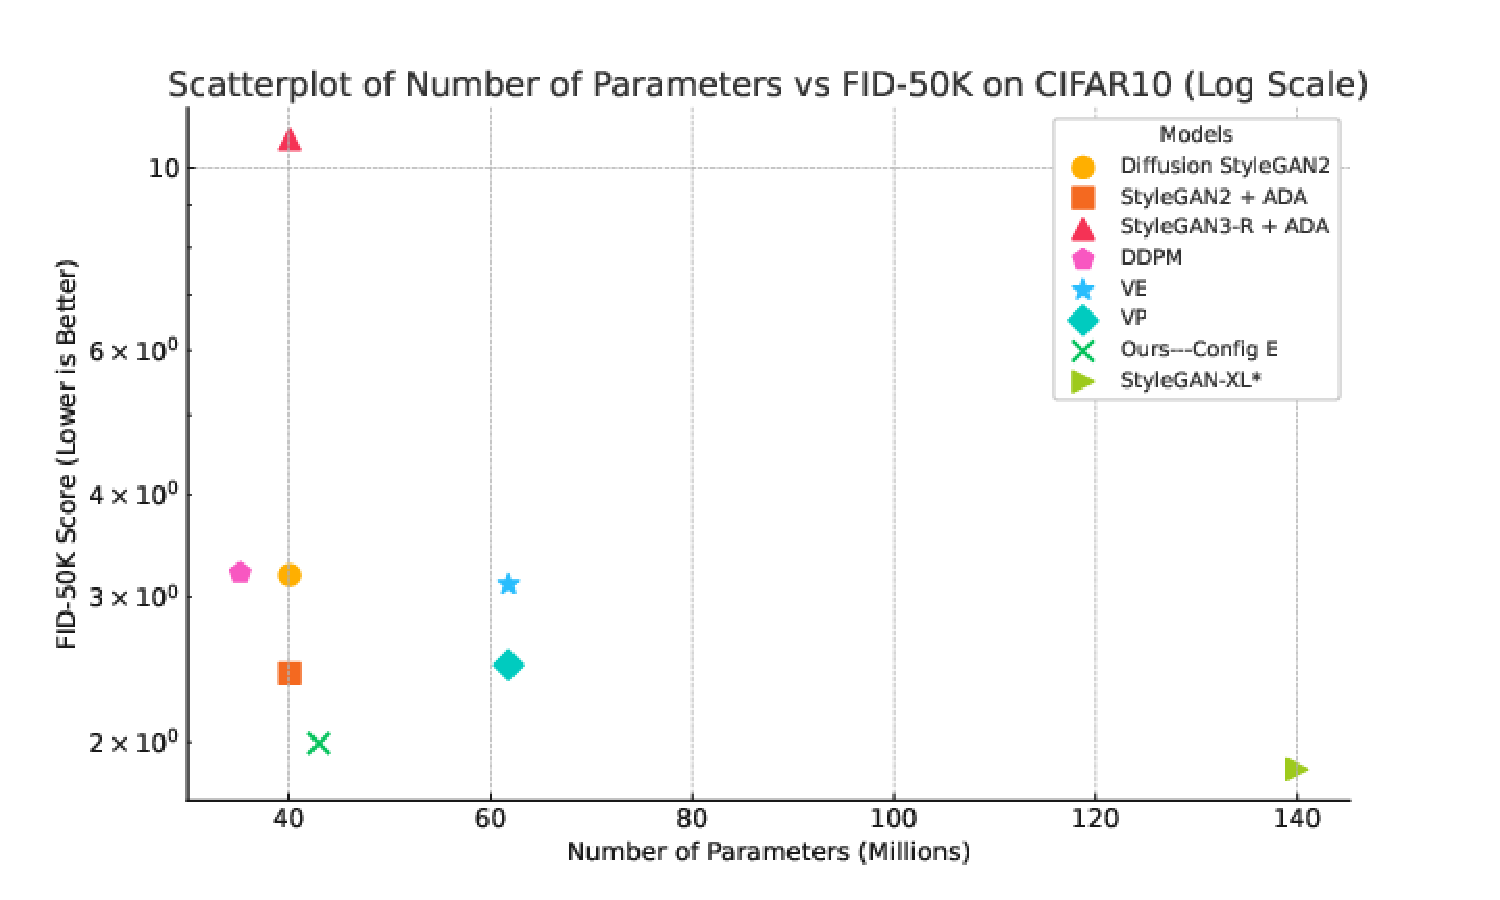
\includegraphics[width=\linewidth,clip,trim={0 0 0 2cm}]{figures/Scatterplot-FID-Parameters-CIFAR10.pdf}
    \caption{Millions of parameters vs.~FID-50K (log scale) on CIFAR-10. Lower is better.}
    \label{fig:fid-50k-vs-params-cifar-10}
\end{wrapfigure}

Many state-of-the-art GANs are derived from Projected GAN~\cite{sauer2021projected}, including StyleGAN-XL~\cite{sgxl} and the concurrent work of StyleSAN-XL~\cite{takida2024san}. These methods use a pre-trained ImageNet classifier in the discriminator. Prior work has shown that a pre-trained ImageNet discriminator can leak ImageNet features into the model~\cite{kynkaanniemi2022role}, causing the model to perform better when evaluating on FID since it relies on a pre-trained ImageNet classifier for the loss. But, this does not improve results in perceptual studies~\cite{kynkaanniemi2022role}. Our model produces its low FID without any ImageNet pre-training.

%\jt{Missing citations here for such methods.}


%\aaron{add NFEs}
%\jt{Which models in our evaluation use this? Any?}

%\jt{What is the second caveat?}

\subsection{FID --- ImageNet-32~\cite{chrabaszcz2017downsampled}}
\label{sec:imagenet32-fid-explain}
We train Config E model until convergence and with optimized hyperparameters and training schedule on ImageNet-32 (conditional generation). We compare against recent GAN models and recent diffusion models in Table~\ref{tab:imagenet32}.
We adjust the number of parameters in the generator of our model to match StyleGAN-XL~\cite{sgxl}'s generator (84M parameters). Specifically, we make the model significantly wider to match. Our method achieves comparable FID despite using a 60\% smaller discriminator (Tab.~\ref{tab:imagenet32}) and despite not using a pre-trained ImageNet classifier.
%, which has been shown to improve FID performance, but not improve results in perceptual studies~\cite{kynkaanniemi2022role}.

\vspace{-0.1cm}
\subsection{FID --- ImageNet-64~\cite{chrabaszcz2017downsampled}}
We evaluate our model on ImageNet-64 to test its scalability. We stack another resolution stage on our ImageNet-32 model, resulting in a generator of 104\ M parameters. This model is nearly 3$\times$ smaller than diffusion-like models~\cite{adm,edm,cm,icm} that rely on the ADM backbone, which contains about 300\ M parameters. Despite the smaller model size and that our model generates samples in one step, it outperforms larger diffusion models with many NFEs on FID (Tab.~\ref{tab:imagenet64}).

\vspace{-0.1cm}
\subsection{Recall}
We evaluate the recall~\cite{precrecall} of our model on each dataset to quantify sample diversity. In general, our model achieves a recall that is similar to or marginally worse than the diffusion model counterpart, yet superior to existing GAN models. For CIFAR-10, the recall of our model peaked at 0.57; as a point of comparison, StyleGAN-XL~\cite{sgxl} has a worse recall of 0.47 despite its lower FID. For FFHQ, we obtain a recall of 0.53 at 64$\times$64 and 0.49 at 256$\times$256, whereas StyleGAN2~\cite{sg2} achieved a recall of 0.43 on FFHQ-256. Our ImageNet-32 model achieved a recall of 0.63; comparable to ADM~\cite{adm}. Our ImageNet-64 model achieved recall 0.59. While this is slightly worse than $\approx$0.63 that many diffusion models achieve, it is better than BigGAN-deep~\cite{biggan} which achieved a recall of 0.48.

\begin{figure}
    \begin{floatrow}
        \capbtabbox{%
        \centering
        \resizebox{0.9\linewidth}{!}{
        \begin{tblr}{
          column{2} = {r},
          column{3} = {r},
          cell{8}{1} = {c=3}{},
          hline{2,7-8} = {-}{},
        }
    Model                                                       & NFE$\downarrow$  & FID$\downarrow$                        \\ 
    DDPM++~\cite{kim2021soft}                  & 1000 & 8.42                                   \\
    VDM~\cite{kingma2021variational}           & 1000 & 7.41                                   \\
    MSGAN~\cite{karnewar2020msg,ning2023input} & 1    & 12.3                                   \\
    ADM~\cite{adm}                             & 1000 & 3.60                                   \\
    DDPM-IP~\cite{ning2023input}               & 1000 & 2.87                                   \\
    Ours—Config E               & 1    & 1.27   \\
    \textit{With ImageNet feature leakage~\cite{kynkaanniemi2022role}:}    \\
    StyleGAN-XL*~\cite{sgxl}                   & 1    & 1.10                                  
    \end{tblr}
        }
    }{%
        \caption{\label{tab:imagenet32}ImageNet-32.}
        % \jt{some are conditional still}}
    }
    %
    \capbtabbox{
        \centering
        \resizebox{0.9\linewidth}{!}{
        \begin{tblr}{
          column{2} = {r},
          column{3} = {r},
          cell{1}{2} = {c},
          cell{1}{3} = {c},
          cell{12}{1} = {c=3}{},
          hline{2-3,11-12} = {-}{},
        }
        Model         & NFE$\downarrow$ & FID$\downarrow$ \\
        BigGAN-deep~\cite{biggan}\phantom{xx}   & 1               & 4.06            \\
        DDPM~\cite{ddpm}          & 250             & 11.0            \\
        DDIM~\cite{ddim}          & 50              & 13.7            \\
        ADM~\cite{adm}           & $^\S$250             & 2.91            \\
        EDM~\cite{edm}           & 79              & 2.23            \\
        CT~\cite{cm}            & 2               & 11.1            \\
        CD~\cite{cm}            & 3               & 4.32            \\
        iCT-deep~\cite{icm}      & 2               & 2.77            \\
        DMD~\cite{dmd}           & 1               & 2.62            \\
        Ours—Config E & 1               & 2.09            \\
        \emph{With ImageNet feature leakage~\cite{kynkaanniemi2022role}:}          &                 &                 \\
        StyleGAN-XL*~\cite{sgxl}   & 1               & 1.52            
        \end{tblr}
        }
    }
    {
        \caption{\label{tab:imagenet64}ImageNet-64.\hspace{-0.1cm} {\small \S:\hspace{-0.05cm}deterministic sampling.}}
    }
    \end{floatrow}
    \vspace{-0.25cm}
\end{figure}


% \begin{table}[ht]
%     \centering
%     \begin{tabular}{lcccccccc}
%         \toprule
%         \textbf{Model} & \textbf{\# Param.} & \textbf{IS $\uparrow$} & \textbf{FID $\downarrow$} & \textbf{Precision $\uparrow$} & \textbf{Recall $\uparrow$} & \textbf{Density $\uparrow$} & \textbf{Coverage $\uparrow$} & \textbf{Inf. (s)} \\
%         \midrule
%         ReACGAN + DiffAug (Ours) [10] & 9.4M & 10.15 & 2.64 & 0.75 & 0.65 & 0.98 & 0.90 & 0.009 \\
%         StyleGAN2-ADA [85] & 20.2M & 10.31 & 2.41 & 0.74 & 0.68 & 1.02 & 0.92 & 0.008 \\
%         StyleGAN2-ADA (Ours) [85] & 20.2M & \textbf{10.53} & 2.31 & 0.75 & 0.69 & 1.04 & 0.93 & 0.008 \\
%         StyleGAN2 + DiffAug + D2D-CE (Ours) [10] & 20.2M & 10.46 & 2.30 & 0.76 & 0.68 & 1.03 & 0.93 & 0.007 \\
%         DDPM [43] & 35.2M & 9.73 & 3.23 & 0.78 & 0.67 & 1.10 & 0.93 & 15.422 \\
%         DDPM++ [44] & 106.6M & 9.90 & 2.49 & 0.78 & 0.69 & 1.12 & 0.94 & 46.697 \\
%         NCSN++ [44] & 107.6M & 10.08 & 2.27 & 0.77 & 0.70 & 1.07 & 0.94 & 99.304 \\
%         LSGM [45] & - & 10.04 & 2.80 & 0.80 & 0.70 & 1.15 & 0.95 & - \\
%         LSGM-ODE [45] & - & 10.07 & \textbf{2.09} & 0.77 & 0.71 & 1.03 & 0.94 & - \\
%         CLD-SGM [47] & - & 9.88 & 2.38 & 0.78 & 0.69 & 1.12 & 0.94 & - \\
%         StyleGAN-XL~ & 18.0M & \textbf{11.03} & \textbf{1.88} & 0.77 & 0.59 & 1.08 & 0.94 & 0.010 \\
%         % BaselineGAN & %10.284011840820312
%         % 10.28
%         % & %1.9925376117527978 
%         % 1.99 & % 0.6899600028991699 
%         % 0.69 &&
%         \bottomrule
%     \end{tabular}
%     \caption{Comparison of various models on CIFAR10 dataset. TODO fix citation}
% \label{tab:cifar10_comparison}
%\end{table}

% \jt{Is the below meant to be a conclusion? Some of these statements are unfounded in the evidence we present so far.}
% \begin{enumerate}

%     \item We demonstrate the ability of our method to recover all modes of training data on Stacked Mnist~\ref{tab:stackedmnist}.
%     \item We beat all methods that do not use bCR (shown to overfit for FFHQ-256~\cite{}) and methods that do not leak imagenet features from a pretrained discriminator~\cite{kynkaanniemi2022role}. If we exclude these two categories of models, we are SOTA across all open source GANs. We also SOTA on a per parameter count basis on multiple GANs.
%     \item We demonstrate SOTA performance on CIFAR-10 image generation at our current parameter count, outperforming all previous GANs except for StyleGAN-XL derived ones with X\% percent of the parameters of these methods. We also do not leak features from ImageNet or use a pretrained discriminator.~\ref{tab:cifar10}. 
%     \item We achieve near SOTA on FFHQ 256 and achieve SOTA for a GAN method without bCR or feature leakage.
%     \item We achieve near state of the art results on Imagenet and achieve Pareto frontier results for total GAN model parameter size.
% \end{enumerate}
% \begin{table}[h]
\centering
\caption{FID on ImageNet-32}
\begin{tabular}{ l c c }
\toprule
Model & \textbf{Year} & FID$\downarrow$ \\
\midrule
% %Real NVP (Dinh et al.) & 2016 & 4.28 \\
% %Glow (Kingma and Dhariwal) & 2018 & 4.09 \\
% %MintNet & 2019 & 4.06 \\
% % Residual Flow & 2019 & 4.01 \\
% % BIVA Maaloe et al. & 2019 & 3.96 \\
% % ANF Huang et al. & 2020 & 3.92 \\
% % NVAE w/ flow & 2020 & 3.92 \\
% % PixelRNN & 2016 & 3.86 \\
% % Flow++ & 2019 & 3.86 \\
% % SPN Menick and Kalchbrenner & 2018 & 3.85 \\
% % Gated PixelCNN & 2016 & 3.83 \\
% % Very Deep VAE & 2020 & 3.8 \\
% % MRCNF & 2021 & 3.77 \\
% % $\delta$-VAE & 2019 & 3.77 \\
% Image Transformer~\cite{parmar2018image} & 2018 & 3.77 \\
% ScoreFlow & 2021 & 3.76 \\
% Reflected Diffusion & 2023 & 3.74 \\
% %Hourglass & 2021 & 3.74 \\
% DenseFlow-74-10 & 2021 & 3.63 \\
% i-DODE & 2023 & 3.43 \\
% MSGAN~\cite{karnewar2020msg} & 2019 & 12.3 \\
% DDPM-IP & 2023 & 2.66 \\
MSGAN~\cite{karnewar2020msg} & 2019 & 12.3 \\
VDM~\cite{kingma2021variational} & 2021 & 7.41 \\
DDPM++~\cite{kim2021soft} & 2021 & 8.42 \\
DDPM-IP~\cite{ning2023input} & 2023 & 2.87 \\
\textbf{Ours} & 2024 & 1.28 \\
StyleGAN-XL~\cite{sauer2022stylegan} & 2022 & \textbf{1.10} \\
\bottomrule
\end{tabular}
\end{table}

% \begin{table}[tO]
%     \centering
%     \begin{tabular}{c|c|c|c}
%          & FID\_50k & Precision & Recall \\
%         StyleGAN &  \\
%         StyleGAN-XL? &
%         Lots of other baselines
%     \end{tabular}
%     \caption{Caption}
%     \label{tab:my_label}
% \end{table}
% \label{sec:exp}
% % cifar10, ffhq, imagenet

% \begin{table}
%     \centering
%     %\caption{Results for CIFAR-10 generation. \aaron{add NFEs}}
%     %\vspace{-2mm}
%     \begin{tblr}{
%       column{2} = {r},
%       cell{1}{2} = {c},
%       hline{2,9,13} = {-}{},
%     }
%     Model               & FID$\downarrow$           \\
%     BigGAN~\cite{biggan}              & 14.73         \\
%     TransGAN~\cite{trans}            & 9.26          \\
%     ViTGAN~\cite{vitgan}              & 6.66          \\
%     DDGAN~\cite{ddgan}               & 3.75          \\
%     Diffusion StyleGAN2 & 3.19          \\
%     StyleGAN2 + ADA     & 2.42          \\
%     StyleGAN3-R + ADA   & 10.83         \\
%     DDPM                & 3.21          \\
%     DDIM                & 4.67          \\
%     VE                  & 3.11          \\
%     VP                  & 2.48          \\
%     Ours---Config E     & \textbf{1.99} 
%     \end{tblr}
%     %\label{tab:cifar10}
%     \caption{Results for CIFAR-10 generation. \aaron{add NFEs}}
%     \label{tab:cifar10}
% \end{table}



%%%%%%%%%%%%%%%%%%%%%%%%%%%%%%%%%%%%%%%%%%%%%%%%%%%%%%%%%%%%%
% Qualitative figures
%%%%%%%%%%%%%%%%%%%%%%%%%%%%%%%%%%%%%%%%%%%%%%%%%%%%%%%%%%%%%

% Variable to control the size of each image
% \begin{figure}
%     \centering
%     \includegraphics{example-image-a}
%     \caption{stacked mnist (qualitative figure) (from powerpoint)}
%     \label{fig:stacked-mnist}
% \end{figure}
% cifar10, ffhq, imagenet

% \noindent\begin{minipage}{.33\textwidth}
% \centering
% \captionof{table}{1000-mode coverage on StackedMNIST.}
% \vspace{-2mm}
% \begin{tblr}{
%   cell{2}{2} = {c},
%   cell{2}{3} = {c},
%   cell{3}{2} = {c},
%   cell{3}{3} = {c},
%   cell{4}{2} = {c},
%   cell{4}{3} = {c},
%   cell{5}{2} = {c},
%   cell{5}{3} = {c},
%   cell{6}{2} = {c},
%   cell{6}{3} = {c},
%   cell{7}{2} = {c},
%   cell{7}{3} = {c},
%   cell{8}{2} = {c},
%   cell{8}{3} = {c},
%   cell{9}{2} = {c},
%   cell{9}{3} = {c},
%   cell{10}{2} = {c},
%   cell{10}{3} = {c},
%   cell{11}{2} = {c},
%   cell{11}{3} = {c},
%   hline{2,11} = {1-3}{},
% }
% Model     & Modes$\uparrow$ & KLD$\downarrow$            &  \\
% DCGAN     & 99            & 3.40\phantom{0}&  \\f
% VEEGAN    & 150           & 2.95\phantom{0}&  \\
% WGAN-GP   & 959           & 0.73\phantom{0}&  \\
% PacGAN    & 992           & 0.28\phantom{0}&  \\
% StyleGAN2 & 940           & 0.42\phantom{0}&  \\
% PresGAN   & \textbf{1000} & 0.12\phantom{0}&  \\
% Adv. DSM  & \textbf{1000} & 1.49\phantom{0}&  \\
% VAEBM     & \textbf{1000} & 0.087          &  \\
% DDGAN     & \textbf{1000} & 0.071          &  \\
% Ours      & \textbf{1000} & \textbf{???} &  
% \end{tblr}
% \label{tab:stackedmnist}
% \end{minipage}%
% \begin{minipage}{.33\textwidth}
% \centering
% \captionof{table}{Results for CIFAR-10 generation.}
% \vspace{-2mm}
% \begin{tblr}{
%   column{2} = {r},
%   cell{1}{2} = {c},
%   hline{2,9,13} = {-}{},
% }
% Model               & FID$\downarrow$           \\
% BigGAN              & 14.73         \\
% TransGAN            & 9.26          \\
% ViTGAN              & 6.66          \\
% DDGAN               & 3.75          \\
% Diffusion StyleGAN2 & 3.19          \\
% StyleGAN2 + ADA     & 2.42          \\
% StyleGAN3-R + ADA   & 10.83         \\
% DDPM                & 3.21          \\
% DDIM                & 4.67          \\
% VE                  & 3.11          \\
% VP                  & 2.48          \\
% Ours                & \textbf{1.99} 
% \end{tblr}
% \label{tab:cifar10}
% \end{minipage}%
% \begin{minipage}{.33\textwidth}
% \centering
% \captionof{table}{Results on FFHQ ($256\times256$).}
% \vspace{-2mm}
% \begin{tblr}{
%   column{2} = {r},
%   cell{1}{2} = {c},
%   hline{2,5} = {-}{},
%   hline{2,9} = {-}{},
% }
% Model       & FID$\downarrow$  \\
% StyleGAN2   & 3.78 \\
% StyleGAN3-T & 4.81 \\
% StyleGAN3-R & 3.92 \\
% LDM & 4.98\\
% ADM (DDIM) & 8.41\\
% ADM (DPM-Solver) & 8.40\\
% Diffusion Autoencoder & 5.81\\
% Ours        & \textbf{2.95} 
% \end{tblr}
% \label{tab:ffhq256}
% \end{minipage}


% \input{tables/cifar10}
% \input{tables/ffhq256}
% \input{tables/MNIST}
\begin{figure}[h!]
    \newlength{\imgsize}
    \setlength{\imgsize}{0.10\linewidth} % Adjust this value to change the size of the images
    
    % New command to include images from a specific directory
    \newcommand{\qualitativeimg}[1]{%
        \includegraphics[width=\imgsize]{figures/qualitative/ffhq-256-000139623/image-#1.jpg}%
    }
    
    \setlength{\tabcolsep}{0pt} % Remove spacing between columns
    \renewcommand{\arraystretch}{0} % Remove spacing between rows
    
    \centering
    \begin{tabular}{cccccccc} % Eight columns
        \qualitativeimg{64} & \qualitativeimg{65} & \qualitativeimg{66} & \qualitativeimg{67} & \qualitativeimg{128} & \qualitativeimg{69} & \qualitativeimg{70} & \qualitativeimg{71} \\
        \qualitativeimg{72} & \qualitativeimg{73} & \qualitativeimg{74} & \qualitativeimg{75} & \qualitativeimg{76} & \qualitativeimg{77} & \qualitativeimg{78} & \qualitativeimg{79} \\
        \qualitativeimg{80} & \qualitativeimg{81} & \qualitativeimg{82} & \qualitativeimg{83} & \qualitativeimg{84} & \qualitativeimg{85} & \qualitativeimg{86} & \qualitativeimg{87} \\
        \qualitativeimg{88} & \qualitativeimg{89} & \qualitativeimg{90} & \qualitativeimg{91} & \qualitativeimg{92} & \qualitativeimg{93} & \qualitativeimg{94} & \qualitativeimg{95} \\
        \qualitativeimg{96} & \qualitativeimg{97} & \qualitativeimg{98} & \qualitativeimg{99} & \qualitativeimg{100} & \qualitativeimg{101} & \qualitativeimg{102} & \qualitativeimg{103} \\
        \qualitativeimg{104} & \qualitativeimg{105} & \qualitativeimg{106} & \qualitativeimg{107} & \qualitativeimg{108} & \qualitativeimg{109} & \qualitativeimg{110} & \qualitativeimg{111} \\
        \qualitativeimg{112} & \qualitativeimg{113} & \qualitativeimg{114} & \qualitativeimg{115} & \qualitativeimg{116} & \qualitativeimg{117} & \qualitativeimg{118} & \qualitativeimg{119} \\
        \qualitativeimg{120} & \qualitativeimg{121} & \qualitativeimg{122} & \qualitativeimg{123} & \qualitativeimg{124} & \qualitativeimg{125} & \qualitativeimg{126} & \qualitativeimg{127} \\
    \end{tabular}
    \caption{Qualitative examples of sample generation from our Config E on FFHQ-256.}
    \label{fig:ffhq-256-teaser}
\end{figure}

	\section{Related work}

There is a rich prior literature on 
probabilistic programming languages (PPLs),
which extend probabilistic graphical models to
support more complex joint distributions whose size and ``shape''
can itself be stochastic (e.g., a graph
unrolled for a random number of iterations,
until a data-dependent stopping criterion is met).
PPLs extend traditional programming languages with the ability to {\it sample} from distributions and {\it observe} values of variables based on data (i.e. condition the model).
The semantics of sample and observe vary depending on the inference algorithm.
For more details, see  \citet{intro_ppl}.

Recently there has been an explosion of interest in large language models, such as 
GPT-3 \citep{gpt3} and PaLM \citep{palm}.
%\citep{lamda}.
These can be used for tasks such as ``zero-shot"
question-answering. In this setting, we 
provide the question $Q$ as a prompt to the LM,
and then sample answers from the model, 
which we denote by $p(A|Q,\theta)$,
where $\theta$ are the pre-trained model parameters.
Alternatively, we can compute the MAP answer,
$\hat{A} = \argmax_A p(A|Q,\theta)$.


To ensure the model ``does the right thing'',
we can provide a small training set of question-answer pairs,
$D = \{ (Q^m,A^m): m=1:M\}$ pairs.
This can be provided as extra context to the model,
provided in the text prompt, followed by sampling
from $p(A|Q,D,\theta)$.
We refer to this as ``few-shot prompting''.
We can also fine-tune the model parameters on $D$ to
get $\theta'$, and then sample
from $p(A|Q,\theta')$.

%We can improve performance on question answering tasks by encouraging the model
%chaining multiple LMs together,  % david: They don't actually do multiple calls, just prompt it to produce the aux variable directly.
%as illustrated in the
%Scratchpad \citep{scratchpads} and Chain of Thought \citep{chainofthought}  papers.
%These papers introduce an  an additional auxiliary ``thought''
%variable $T$ and then extend the model to have the form
%$P(A,T|Q) = P(A|T,Q)P(T|Q)$, where each conditional is computed
%using an LM.

We can improve performance by introducing an additional auxiliary ``thought'' variable,
and then extend the model to have the form $p(A,T|Q) = p(A|T,Q)p(T|Q)$, where each conditional is computed using an LM which includes its conditioning variables as a part of its input.
Work on scratchpads \citep{scratchpads} and chain of thought \citep{chainofthought} illustrate this, and finetune or prompt the LM to produce this auxiliary thought before answering.
%We can improve performance on question answering tasks by encouraging the model
%chaining multiple LMs together,  % david: They don't actually do multiple calls, just prompt it to produce the aux variable directly.
% These papers 
% variable $T$ 

We typically condition this on a small set
$D_S$ of  $(A^m,T^m,Q^m)$ triples,
and optionally a larger set $D_L$ of $(A^m, Q^m)$ pairs.
We then compute a distribution over answers to a test question
using
\begin{align}
\hat{p}(A|Q) = \sum_T 
\hat{p}(A|Q, T) \hat{p}(T|Q)
\label{eqn:probQA}
\end{align}
where $\hat{p}(\cdot) = p(\cdot|D_L,D_S,\theta)$
is the prior predictive distribution. (Scratchpad creates its prior predictive by fine-tuning, while Chain of Thought adds $D_S$ to the LM prompt.)

In practice, we cannot sum over all possible strings $T$
in \cref{eqn:probQA}.
The most common approach is to compute the MAP estimate
$\hat{T} = \argmax \hat{p}(T)$ using beam search,
and then to approximate the sum over $T$ with this single
value.
More recently, Self Consistency \citep{selfconsistency} 
proposed to sample multiple values for $T$
using forward sampling of $(A,T)$ given $Q$,
and then taking the answer $A$ that is most common
in this set\footnote{This bucketing is practical because most standard benchmarks have answers that are just a couple words.}.

PromptChainer \citep{promptchainer} proposes a visual interface for composing language models together, specifying control flow and prompting strategies for each node in a chain. Nodes may query language models or external systems. 
Socratic models \citep{socraticmodels} extends model chaining to the multimodal setting and demonstrates zero-shot abilities on tasks for which no single model exists.

The Eliciting Latent Knowledge proposal \citep{ELK} suggests making latent variables explicit, modelled using a Bayesian network, to improve interpretability and safety for advanced AI systems.
% Factored cognition \citet{factored_cognition}

\citet{ortega2021shaking} explains a formalism for LM finetuning with causal graphical models in order to extend the predictive capabilities of AI agents towards more adaptive behaviour. They focus on analysing an auto-regressive action (random variable) prediction scheme in the interactive setting of RL where a model is simultaneously a generator and predictor of data.

% \citet{language_feedback} incorporates language feedback to finetune models, and finds that learning is significantly more sample efficient. \ddohan{We view this feedback as an auxiliary variable which can be conditioned to inform inference.}

%\kevin{Omit RL refs since not relevant?}
%Incorporating human feedback into generative models remains an open problem. Reinforcement from human feedback has become a popular approach to finetuning models against human preferences. \citep{learning_to_summarize, anthropic_human_feedback} learn a surrogate model of human preferences and use PPO \citep{ppo} to finetune a language model to maximize this surrogate. Rather than using scalar feedback, \citet{language_feedback} incorporates language feedback to finetune models, and finds that learning is significantly more sample efficient. \ddohan{We view this feedback as an auxiliary variable which can be conditioned to inform inference.}
%\todo{ddohan: consider adding back in language feedback ref}

%\citep{Levine2022} presents some very recent work on using frozen LMs in various ways.\rif{Suggest we cut this if we don't have more to say.}






    \section{Conclusion}
\label{sec:conclusion}
This paper introduced \tool, a language to describe distributed machine learning workloads and optimize them across computation and communication boundary. 
We show that \tool{} generated code significantly improves several training and inference times of large language models. 
In the future we plan to automate the optimizations through smart search.

% With ever increasing larger models being trained on massively
% distributed clusters using large datasets, there is a need for
% optimized communication and computation kernels.  Existing techniques
% to improve data-parallel and model-parallel training are limited to a
% particular algorithm, which might not be optimal for different input
% tensor sizes, topology of a distributed system.  In this paper, we
% presented \tool DSL to express programs that contains communication
% and computation and several transformations to optimize these programs
% for wide range of scenarios.  Code generated by \tool performs
% significantly better than hand-optimized state-of-the-arts.

    {\small
        \bibliography{mixup}
        \bibliographystyle{iclr2018}}
\end{document}
